\documentclass[11pt]{article}
\usepackage[margin=1in]{geometry}
\usepackage{amsmath,amssymb,amsthm}
\usepackage{booktabs}
\usepackage{array}
\usepackage{enumitem}
\usepackage{xcolor}
\usepackage{hyperref}
\hypersetup{colorlinks=true,linkcolor=blue!50!black,urlcolor=blue!50!black,citecolor=blue!50!black}
\usepackage{listings}
\usepackage[protrusion=true,expansion=false]{microtype}
\usepackage{pgfplots}
\pgfplotsset{compat=1.17}
\usetikzlibrary{patterns}

\lstset{
  basicstyle=\ttfamily\footnotesize,
  breaklines=true,
  frame=single,
  framesep=4pt,
  backgroundcolor=\color{gray!6},
  columns=fullflexible,
  keepspaces=true,
  numbers=left,
  numberstyle=\tiny\color{gray!70},
  language=Java,
  morekeywords={const,let,function,return,export,interface,type,readonly,for,if,else,throw,new},
}

\newtheorem{proposition}{Proposition}
\newtheorem{definition}{Definition}
\newtheorem{corollary}{Corollary}
\theoremstyle{remark}
\newtheorem{remark}{Remark}
\newcommand{\tier}[1]{\textsc{\MakeLowercase{#1}}}
\pgfplotsset{
  floorplot/.style={
    width=0.92\linewidth, height=5.6cm, grid=both,
    grid style={line width=.2pt, draw=gray!22},
    major grid style={line width=.2pt,draw=gray!40},
    tick align=outside, tick pos=left,
    legend cell align=left, legend style={font=\footnotesize, draw=gray!40},
  },
}

%%% ---- figure data, emitted by scripts/paper-figures.mts ------------------
\newcommand{\fighystUp}{coordinates {(2.2,1.000000) (2.3,1.000000) (2.4,1.000000) (2.5,1.000000) (2.6,1.000000) (2.7,1.000000) (2.8,1.000000) (2.9,0.999999) (3,0.999947) (3.1,0.265109) (3.2,0.225650) (3.3,0.215639) (3.4,0.206601) (3.5,0.198426) (3.6,0.190984) (3.7,0.184160) (3.8,0.177879)}}
\newcommand{\fighystDn}{coordinates {(2.2,0.999944) (2.3,0.999932) (2.4,0.899820) (2.5,0.652800) (2.6,0.574077) (2.7,0.478750) (2.8,0.422302) (2.9,0.346650) (3,0.250000) (3.1,0.237054) (3.2,0.225708) (3.3,0.215635) (3.4,0.206600) (3.5,0.198428) (3.6,0.190983) (3.7,0.184161) (3.8,0.177878)}}
\newcommand{\figctrlUp}{coordinates {(0.6,1.000000) (0.7,1.000000) (0.8,1.000000) (0.9,0.999999) (1,0.999948) (1.1,0.931713) (1.2,0.833446) (1.3,0.769230) (1.4,0.714285) (1.5,0.666667) (1.6,0.625000) (1.7,0.588235) (1.8,0.555556) (1.9,0.526316) (2,0.500000) (2.1,0.476191) (2.2,0.454545)}}
\newcommand{\figctrlDn}{coordinates {(0.6,0.999869) (0.7,0.999735) (0.8,0.999277) (0.9,0.997381) (1,0.982126) (1.1,0.909141) (1.2,0.833336) (1.3,0.769231) (1.4,0.714286) (1.5,0.666667) (1.6,0.625000) (1.7,0.588235) (1.8,0.555556) (1.9,0.526316) (2,0.500000) (2.1,0.476190) (2.2,0.454545)}}
\newcommand{\figcoex}{coordinates {(1,0.05342509) (2,0.05342509) (3,0.05342509) (4,0.05342509) (5,0.05342509) (6,0.05342509) (7,0.05342509) (8,0.05342509) (9,0.05342509) (10,0.05342509) (11,0.05342509) (12,0.05342509) (13,0.05342509) (14,0.05342509) (15,0.05342509) (16,0.05342509) (17,0.05342509) (18,0.05342509) (19,0.05342509) (20,0.05342509) (21,0.05342509) (22,0.05342509) (23,0.05342509) (24,0.05342509) (25,0.05342509) (26,0.05342509) (27,0.05342509) (28,0.05342509) (29,1.00000000) (30,1.00000000) (31,1.00000000) (32,1.00000000) (33,1.00000000) (34,1.00000000) (35,1.00000000) (36,1.00000000)}}
\newcommand{\coexFar}{0.05342509}
\newcommand{\coexMean}{0.263775}
\newcommand{\coexNfar}{28}
\newcommand{\coexNflat}{8}

\newcommand{\figquartic}{coordinates {(0.32,1.374572e-3) (0.16,8.612204e-5) (0.08,5.380303e-6) (0.04,3.360571e-7) (0.02,2.099478e-8) (0.01,1.311865e-9)}}
\newcommand{\nZeros}{2003}
\newcommand{\nGrid}{29456}
\newcommand{\corrBase}{0.8362}

\newcommand{\figgibbsAway}{coordinates {(0,0.789503) (0.05,0.884186) (0.1,0.936208) (0.15,0.956340) (0.2,0.959264) (0.25,0.954590) (0.3,0.948792) (0.4,0.943778)}}
\newcommand{\figgibbsNear}{coordinates {(0.05,0.399888) (0.1,0.556649) (0.15,0.652832) (0.2,0.704550) (0.25,0.733806) (0.3,0.750710) (0.4,0.769757)}}
\newcommand{\figscaleRaw300}{coordinates {(330,0.755132) (900,0.707437) (1500,0.679188) (2157,0.672849)}}
\newcommand{\figscaleRaw1000}{coordinates {(330,0.797381) (900,0.759281) (1500,0.740686) (2157,0.732051)}}
\newcommand{\figscaleRaw3000}{coordinates {(330,0.825240) (900,0.793595) (1500,0.779241) (2157,0.771282)}}
\newcommand{\figscaleMsk300}{coordinates {(330,0.951481) (900,0.937529) (1500,0.922749) (2157,0.914845)}}
\newcommand{\figscaleMsk1000}{coordinates {(330,0.957881) (900,0.955732) (1500,0.950558) (2157,0.945962)}}
\newcommand{\figscaleMsk3000}{coordinates {(330,0.960852) (900,0.960723) (1500,0.958836) (2157,0.957771)}}
\newcommand{\figamplMine}{coordinates {(2003,499.8)}}
\newcommand{\figamplPub}{coordinates {(20000,3030) (100000,11497)}}
\newcommand{\amplExp}{0.829}
\newcommand{\amplPred}{450}


%%% -------------------------------------------------------------------------

\title{\textbf{Instrument Floors}\\[3pt]
\large Three criteria for what a finite measurement determines,\\
with instruments and results on lattice $SU(2)$ and the zeros of $\zeta$}
\author{\small Agent record, 21 October 2026. Byline unset --- see \textbf{Contributions}.\\
\small Prior instrument: B.\ Wallace (TensorRent), FF06e.}
\date{}

\begin{document}
\maketitle

\begin{abstract}
A finite battery of statistics applied to an object answers fewer questions than it
appears to. We give three criteria for separating what a measurement determines from
what its instrument contributed, state each as a proposition, build the instrument that
tests it, and measure the result on two objects sharing no subject matter. \textbf{(I)
Descent.} A surrogate construction is a choice of quotient $\pi\colon X\to X/G$; a
statistic either factors through $\pi$ or sees the fibre. Factoring statistics have a
degenerate null distribution, so their standardised significance is $0/0$ rather than
small; bounded statistics have a reachable ceiling on significance, below which no
object can be convicted; and non-factoring is necessary but not sufficient for
detection. A four-tier verdict follows. Applied to a $6\times6$ Wilson $SU(2)$
configuration, a battery of six statistics is shown to carry at most three independent
readings. \textbf{(II) Linear invisibility in parameter space.} For a lattice action
built from three $SU(2)$ characters, the entire quadratic fluctuation spectrum about
the flat vacuum depends on one combination $c_1=\beta-2\alpha+5\lambda$ of the three
couplings; higher terms first enter at \emph{quartic} order in the field. Two actions
sharing $c_1$ are therefore indistinguishable to every linear measurement while
differing in vacuum count --- measured, with the discrepancy scaling as amplitude$^4$
over three halvings. \textbf{(III) Localisation.} A residual can be attributed to
instrument truncation rather than to missing structure by masking the neighbourhoods
where truncation rings and re-measuring. On the counting fluctuation of the Riemann
zeros, explained variance rises from $0.790$ to $0.959$ on excluding points within a
fifth of a mean spacing of a zero, while the excluded points fall to $0.400$: the
residual is instrument. The same mechanism accounts for an apparent loss of
scale-stability, which becomes a decline of $0.003$ over a fourfold range in height
once the neighbourhoods are removed. Along the way the cubic character produces a
first-order transition in the lattice with a measured hysteresis loop and two-phase
coexistence at the predicted root, and we localise a known $0.4$--$1.0\sigma$ artifact
in a published surrogate pipeline to piecewise-linear interpolation specifically, which
makes it removable. All instruments are anchored on values they were not tuned to, and
every figure is emitted from the measurement that produced it.
\end{abstract}

\begin{center}\small\fbox{\begin{minipage}{0.92\linewidth}
\textbf{Status in this repository.} A supporting document under \path{docs/},
outside the 35-paper canonical publication inventory and its build job, following the
placement of the Yang--Mills comparison methodology paper. Its propositions and
measurements are not part of the corpus author statement; see \textbf{Contributions} on
the final page. Figures are generated by the script named in \S\ref{sec:repro} into
\texttt{instrument\_floors\_data.tex}, which this document \texttt{\textbackslash input}s.
\end{minipage}}\end{center}

\section{Claim boundaries}\label{sec:status}

Status is separated from exposition. No claim is stated more strongly in the text than
here.

\begin{center}\small
\begin{tabular}{p{0.46\linewidth}ll}
\toprule
Claim & Status & Where \\
\midrule
Props.~\ref{prop:degenerate}--\ref{prop:necessary}, \ref{prop:c1}, \ref{prop:ceiling2} & elementary, proved & \S\ref{sec:descent}, \S\ref{sec:invis} \\
Six lattice statistics carry $\le3$ readings & measured; 4 of 4 collapses structural & \S\ref{sec:battery} \\
Equal $c_1$ hides a different vacuum count & measured; scaling exponent $4$ confirmed & \S\ref{sec:invis} \\
First-order transition at $\rho=1+5\lambda/\beta$ & measured: loop, coexistence, spinodal & \S\ref{sec:firstorder} \\
The $\zeta$ residual is truncation, not structure & measured, one masking family & \S\ref{sec:gibbs} \\
Scale-stability holds after masking & measured, four windows & \S\ref{sec:gibbs} \\
The $0.4$--$1.0\sigma$ artifact needs linear interpolation & measured, one implementation & \S\ref{sec:artifact} \\
Amplification: our point near the published curve & measured; $11\%$ high, two-point fit & \S\ref{sec:zresults} \\
Any claim about $\zeta$, RH, or continuum $SU(2)$ & \textbf{none made} & \S\ref{sec:scope} \\
\bottomrule
\end{tabular}
\end{center}

\section{Introduction}

An object admits no shortage of statistics, and when many of them behave as expected the
usual reading is over-determination. The opposite reading is available on the same
evidence: if the statistics are not independent, their agreement is redundancy, and if
what they share is generic to a class rather than specific to the object, their
convergence reports only class membership --- true of uncountably many objects with
nothing else in common.

That is one instance of a general problem. A measurement's output is a composite of the
object and the instrument, and the instrument's contribution is itself a quantity to be
measured rather than assumed small. Three cases arise repeatedly and admit sharp
criteria:

\begin{enumerate}[leftmargin=2em,itemsep=2pt]
\item A statistic may be \emph{determined by a coarsening} of the object, so that it
      cannot distinguish the object from anything else with the same coarse data
      (\S\ref{sec:descent}).
\item A \emph{parameter} of a model may be invisible to the order of response one is
      measuring, so that distinct models are indistinguishable by that measurement and
      differ elsewhere (\S\ref{sec:invis}).
\item A \emph{residual} may be produced by the truncation of the instrument rather than
      by structure the model fails to reach, and the two are separable by where the
      residual lives (\S\ref{sec:gibbs}).
\end{enumerate}

Each section below states the criterion, builds the instrument, anchors it, and reports
what it measured. The two objects are a finite Wilson $SU(2)$ lattice gauge
configuration and the first $\nZeros$ non-trivial zeros of $\zeta$, chosen because they
share no subject matter: a criterion validated on one object is accommodated to it.

Criterion~I is an amendment to an existing instrument \cite{ff06e}, itself a
specialisation of surrogate-data testing \cite{theiler}; criteria II and III are built
here. None of the propositions is deep. The contribution is that each is omitted in
practice, together with the measured size of the omission.

\section{Criterion I: descent}\label{sec:descent}

\subsection{Framework}

\begin{definition}[Quotient, surrogate]
Let the object $X$ decompose into components $x_1,\dots,x_n$ and let $G=S_n$ act by
permuting them. Write $\pi\colon X\mapsto X/G$ for the orbit map, which sends an object
to its multiset of components --- equivalently, to its one-point distribution, or
\emph{marginal}. A \emph{surrogate} is $gX$ for $g$ drawn uniformly from $G$: identical
marginal, no higher structure of $X$'s.
\end{definition}

\begin{definition}[Witness, significance, factoring]
A \emph{witness} is $W\colon X\mapsto\mathbb{R}$. Over an ensemble of $K$ surrogates
with mean $\overline{W}$ and standard deviation $\sigma_W$, the \emph{standardised
significance} is $z(W)=|W(X)-\overline{W}|/\sigma_W$. $W$ \emph{factors through the
marginal} if $W=\widetilde{W}\circ\pi$ for some $\widetilde{W}$, equivalently if
$W(gX)=W(X)$ for all $g\in G$.
\end{definition}

The existing criterion \cite{ff06e} declares $W$ \emph{form} when $z$ is small
($\lesssim3$) and \emph{function} when large, reading the first as evidence that $W$
responds to the class and the second that it responds to the object. The quotient
language makes the content plain: a form witness is one determined by $\pi$, and the
surrogate destroys exactly the fibre. This is a descent question, and it makes the first
proposition a corollary rather than a finding.

\subsection{Three propositions}

\begin{proposition}[Degenerate null]\label{prop:degenerate}
If $W$ factors through the marginal, the null distribution of $W$ is $\delta_{W(X)}$.
Hence $\overline{W}=W(X)$, $\sigma_W=0$, and $z(W)=0/0$ is undefined.
\end{proposition}
\begin{proof}
$W(gX)=W(X)$ for all $g\in G$, so the pushforward of any measure on $G$ under
$g\mapsto W(gX)$ is the point mass at $W(X)$.
\end{proof}

\begin{corollary}
A reported small $z$ for a factoring witness is not a small effect. Evaluated in
floating point, $0/0$ returns the residue of summation order. Measured on the lattice of
\S\ref{sec:lattice}, where the mean of $\operatorname{Re}U$ over links is a symmetric
function of the link multiset: $\sigma_W=6.5\times10^{-16}$ and the computed $z$ is
$1.4$.
\end{corollary}

\begin{proposition}[Reachable ceiling]\label{prop:ceiling}
Let $W$ take values in $[a,b]$ with null mean $\mu$ and $\sigma_W>0$. For every object
with that null,
\[
  z(W)\;\le\;C(W)\;:=\;\frac{\max(b-\mu,\;\mu-a)}{\sigma_W}.
\]
If $C(W)<\tau$ for threshold $\tau$, no object attains $z\ge\tau$.
\end{proposition}
\begin{proof}
$|W(X')-\mu|\le\max(b-\mu,\mu-a)$ since $W(X')\in[a,b]$.
\end{proof}

A low $z$ from such a witness is a statement about resolution; calling it \emph{form}
attributes to the object what belongs to the test. Measured: a Wilson loop trace on a
$6\times6$ lattice, range $[-1,1]$, has $\sigma_W\in[0.11,0.45]$, giving $C<5$ and in
places $C<2$ against $\tau=3$.

\begin{proposition}[Non-factoring is not sufficient]\label{prop:necessary}
Non-factoring is necessary for $\sigma_W>0$ but does not imply $W(X)$ is separated from
the null: there are non-factoring $W$ and objects $X$ with $z(W)$ arbitrarily small.
\end{proposition}
\begin{proof}
Let $W(x)=\#\{i:x_{i+1}>x_i\}$, which does not factor. For $X$ a discretised sine period
of length $n$ the sequence ascends on half its period, so $W(X)\approx n/2$, while the
null mean is $(n-1)/2$. At $n=60$: $W(X)\in\{29,30\}$, null mean $29.5$, $z=0.34$. The
same $W$ on a monotone sequence gives $W=n-1$ and large $z$.
\end{proof}

Hence \emph{form} is a property of the pair $(W,X)$, never of $W$. The practical
consequence is a reading of \cite{ff06e}'s own results: its distributional witnesses are
form \emph{on the zeros}, which is what was measured, and are serviceable statistics on
objects whose marginal does not determine them.

\begin{remark}
None of the three is novel as statistics: a permutation test needs a statistic that
varies under the null, and any test needs power. The single error behind all three is
conflating ``does not factor'' with ``detects''.
\end{remark}

\subsection{The decision procedure}

\begin{lstlisting}[caption={The four-tier verdict (abridged from \texttt{src/shuffle-knife.ts}). \texttt{floor} is scaled to the witness magnitude; \texttt{range} is present only for bounded witnesses.},label={lst:knife}]
const floor = 1e-12 * Math.max(1, Math.abs(real));
const worst = Math.max(...vals.map((x) => Math.abs(x - real)));

// (1) structural: every surrogate IS the object, so there is no statistic
if (worst <= floor) return { tier: "FORM_EXACT", z: null, ceiling: null };

// every surrogate agrees with every other but not with the object
if (sd <= floor) return { tier: "FUNCTION", z: Infinity, ceiling: null };

const ceiling = w.range ? Math.max(w.range[1] - mean, mean - w.range[0]) / sd : null;
const z = Math.abs(real - mean) / sd;

// (2) the witness could not have reached the bar, so its z is not evidence
if (ceiling !== null && ceiling < threshold) return { tier: "NO_POWER", z, ceiling };

// (3) a verdict about THIS pair, not about the witness
return { tier: z >= threshold ? "FUNCTION" : "FORM", z, ceiling };
\end{lstlisting}

A separate check catches a different redundancy: witnesses pairwise affine across three
or more objects are one witness twice, and counting both double-counts.

\subsection{Calibration is a precondition}\label{sec:calib}

The caller supplies the surrogate construction, because only the caller knows what the
marginal is; this is the one irreducibly domain-specific choice. If the construction
fails to preserve the marginal it is randomisation, and then every witness reads
\tier{FUNCTION} for a reason unrelated to the object. \emph{No internal check detects
this and nothing about the output looks wrong.} Measured: replacing the permutation with
fresh random values convicts the sample variance --- a provable invariant --- as
\tier{FUNCTION}. The only detector is the requirement that a known invariant return
\tier{FORM\_EXACT}, which is why calibration is a precondition rather than good practice.

The implemented protocol: known invariants must read \tier{FORM\_EXACT} with $z$
withheld; known non-factoring witnesses on a structured object must read
\tier{FUNCTION}; a decoy independent of the object must not read \tier{FUNCTION}; a
deliberately marginal-breaking surrogate must convict an invariant; fewer than two
surrogates must refuse to run.

\section{The lattice instrument}\label{sec:lattice}

A $W\times W$ periodic lattice carries $U\in SU(2)$ on each link as a unit quaternion
\cite{wilson}. The marginal is the multiset of link rotors; the surrogate permutes which
site each link occupies. Spatial adjacency is what gauge structure consists of --- a
plaquette being the ordered product around a face --- so adjacency is the structure the
surrogate must destroy.

\subsection{A three-character action}

Let $w=\tfrac12\operatorname{tr}P$ for a plaquette $P$. The $SU(2)$ characters
$\chi_{1/2}=2w$, $\chi_1=4w^2-1$ and $\chi_{3/2}=8w^3-4w$ give, normalised to unity at
the identity, a per-face potential
\begin{equation}\label{eq:action}
  g(w)\;=\;\underbrace{\beta(1-w)}_{\text{fundamental}}
          \;-\;\underbrace{\alpha(1-w^2)}_{\text{adjoint}}
          \;+\;\underbrace{\lambda\bigl(1-(2w^3-w)\bigr)}_{j=3/2},
  \qquad V=\sum_{\text{faces}}g(w_P).
\end{equation}
In the order parameter $m=1-w$ this is $c_1m+c_2m^2+c_3m^3$ with
\begin{equation}\label{eq:cs}
  c_1=\beta-2\alpha+5\lambda,\qquad c_2=\alpha-6\lambda,\qquad c_3=2\lambda.
\end{equation}
A single sign of $\lambda$ therefore raises $c_1$, drives $c_2$ through zero and
supplies $c_3>0$: the three things a first-order transition requires, with no shape
fitted.

Every term is a different weight on one staple, which is why the force is one
expression. For $V=\sum g(w_P)$,
\begin{equation}\label{eq:force}
  F \;=\; \mathrm{vec}\Bigl(U\cdot\textstyle\sum_{\text{faces}}g'(w_P)\,s_{\text{face}}\Bigr),
  \qquad g'(w)=-\beta+2\alpha w+\lambda(1-6w^2),
\end{equation}
since $\sum\partial w_P/\partial U=-\mathrm{vec}(U s_{\text{face}})$. The sign of
$g'(1)=-\beta+2\alpha-5\lambda$ reads the stability of the flat vacuum directly.

\begin{lstlisting}[caption={The force (abridged from \texttt{src/rotor-dynamics.ts}), with the pure-Wilson fast path retained so $\alpha=\lambda=0$ is bit-identical to the prior organ.},label={lst:force}]
export const faceWeight = (w, beta, alpha, lambda) =>
  -beta + 2 * alpha * w + lambda * (1 - 6 * w * w);

export function force(f, a, x, y, beta, alpha = 0, lambda = 0) {
  const u = getLink(f, a, x, y);
  if (alpha === 0 && lambda === 0) {            // every face carries one weight
    const v = vec(mul(u, staple(f, a, x, y)));
    return [-beta * v[0], -beta * v[1], -beta * v[2]];
  }
  const pair = staplePair(f, a, x, y);          // each face weighted at ITS own w
  const k0 = faceWeight(pair[0].w, beta, alpha, lambda);
  const k1 = faceWeight(pair[1].w, beta, alpha, lambda);
  const aw = [0,1,2,3].map((i) => k0 * pair[0].s[i] + k1 * pair[1].s[i]);
  return vec(mul(u, aw));
}
\end{lstlisting}

\subsection{Validation}

Equation~\eqref{eq:force} is checked against a central finite difference of $V$ rather
than against its derivation, at four $(\alpha,\lambda)$ pairs including a negative
$\lambda$ --- a sign error cancelling for one sign would not survive both. Worst
disagreement $2.4\times10^{-9}$ at $\epsilon=10^{-6}$. Dynamics are BAOAB Langevin; at
$\gamma=0,T=0$ the integrator reproduces leapfrog to machine epsilon, and the position
update being a group multiplication, $\|U\|=1$ survives without renormalisation.

Four mutations of \eqref{eq:action}--\eqref{eq:force} were introduced and all are
caught, with an informative split: mutants in $g'$ kill seven tests by changing the
dynamics, while mutants in $V$ kill exactly one --- the finite-difference check ---
because a potential/force mismatch is invisible to any sweep of the dynamics.

\section{Criterion II: linear invisibility in parameter space}\label{sec:invis}

\begin{proposition}[The quadratic spectrum sees one combination]\label{prop:c1}
Near the flat vacuum, $m_P=1-w_P=\tfrac12|v_P|^2+O(|v|^4)$ where $v_P$ is the
plaquette's algebra vector. Hence
\[
  V \;=\; \frac{c_1}{2}\sum_P |v_P|^2 \;+\; O(|v|^4),
\]
so the entire linearised fluctuation spectrum --- every $\omega(k)$, the whole
small-amplitude response --- is fixed by $c_1=\beta-2\alpha+5\lambda$ alone, and $c_2$,
$c_3$ first enter at \emph{quartic} order in the field.
\end{proposition}
\begin{proof}
$m$ is already quadratic in the fluctuation, so $c_2m^2$ and $c_3m^3$ are quartic and
sextic.
\end{proof}

\begin{proposition}[Degeneracy]\label{prop:ceiling2}
The family $\{(\beta,\alpha,\lambda):\beta-2\alpha+5\lambda=c_1\}$ is two-dimensional.
Any two of its members are indistinguishable to every measurement of quadratic response
about the flat vacuum, and may differ in the number of minima of $g$, since that is
governed by $c_2^2>3c_1c_3$ with $c_2<0$.
\end{proposition}

\paragraph{Measured.} Take $c_1=\tfrac12$ for both:
\[
  A=(\beta,\alpha,\lambda)=(0.5,\,0,\,0), \qquad B=(0.5,\,1.0,\,0.4).
\]
$A$ is pure Wilson with one minimum; $B$ has $c_2=-1.4$, $c_3=0.8$, hence
$c_2^2=1.96>3c_1c_3=1.2$: two minima, the flat one metastable. Figure~\ref{fig:quartic}
measures the blindness as a \emph{scaling exponent} rather than a tolerance.

\begin{figure}[ht]\centering
\begin{tikzpicture}
\begin{loglogaxis}[floorplot, xlabel={fluctuation amplitude}, ylabel={$|V_A-V_B|$},
  legend pos=north west, height=5.2cm]
\addplot[mark=*, thick, color=blue!60!black] coordinates {\figquartic};
\addlegendentry{measured}
\addplot[domain=0.01:0.32, samples=2, dashed, thick, color=red!60!black, forget plot]
  {0.1312*x^4};
\node[anchor=west, font=\footnotesize, color=red!60!black] at (axis cs:0.02,4e-7) {slope $4$};
\end{loglogaxis}
\end{tikzpicture}
\caption{Two actions sharing $c_1$ disagree only at quartic order. Halving the amplitude
divides the discrepancy by $16.0$ at each of three successive halvings, and
$|V_A-V_B|/\text{amp}^4$ is constant at $0.131$. \emph{Falsifier:} a quadratic
disagreement would give a factor of $4$. Breaking $c_1$ by $4\%$ ($\beta=0.5\to0.52$)
moves the measured exponent from $16.0$ to $4.0$ --- exactly quartic to quadratic ---
so the test detects the degeneracy's absence by kind, not by magnitude.}
\label{fig:quartic}
\end{figure}

Relaxed from the flat vacuum both actions give $1.000000$. Relaxed from the far basin,
$A$ returns to flat ($0.999881$) and $B$ does not ($0.263775$). \emph{Identical linear
response, different vacuum count}, and the only measurement that separates them is one
started in the other basin.

\section{A first-order transition}\label{sec:firstorder}

The transition the cubic creates was pre-registered before measurement, including the
metric and its kill condition, because the obvious metric is the wrong one: the largest
step in a swept order parameter cannot distinguish a discontinuity from a steeper
continuous curve, being a function of the sweep resolution. At $\lambda=0$ the same
curve reads $0.098$ on a grid of $0.1$ and $0.167$ on a coarser one.

The discriminant is \emph{hysteresis}. A damped relaxation sits in whichever minimum it
started nearest until that minimum stops \emph{existing} --- the spinodal --- not until
it stops being global, so two minima make the up- and down-sweeps disagree and one
minimum cannot, at any steepness.

\begin{figure}[ht]\centering
\begin{tikzpicture}
\begin{axis}[floorplot, width=0.48\linewidth, height=5.2cm,
  xlabel={$\rho=2\alpha/\beta$}, ylabel={$\langle\operatorname{Re}P\rangle$},
  title={\footnotesize $\lambda=0.4$: a loop}, legend pos=south west,
  ymin=0, ymax=1.08, legend style={font=\scriptsize, draw=gray!40}]
\addplot[mark=*, thick, color=blue!60!black] coordinates {\fighystUp};  \addlegendentry{from flat}
\addplot[mark=square*, thick, color=orange!80!black] coordinates {\fighystDn}; \addlegendentry{from the far basin}
\draw[dashed, gray] (axis cs:3,0) -- (axis cs:3,1.08);
\node[anchor=south, font=\scriptsize, color=gray!50!black, rotate=90] at (axis cs:2.96,0.1)
  {$\rho=1+5\lambda/\beta$};
\draw[<->, thick, color=red!60!black] (axis cs:3,0.999947) -- (axis cs:3,0.250000);
\node[anchor=west, font=\footnotesize, color=red!60!black] at (axis cs:3.04,0.62) {$0.7499$};
\end{axis}
\begin{axis}[floorplot, width=0.48\linewidth, height=5.2cm, at={(0.52\linewidth,0)},
  xlabel={$\rho=2\alpha/\beta$}, title={\footnotesize $\lambda=0$ control: no loop},
  ymin=0, ymax=1.08, yticklabel pos=right]
\addplot[mark=*, thick, color=blue!60!black] coordinates {\figctrlUp};
\addplot[mark=square*, thick, color=orange!80!black] coordinates {\figctrlDn};
\node[anchor=north east, font=\scriptsize, color=gray!50!black, align=right]
  at (axis cs:2.2,1.04) {branches coincide\\gap $0.0226$};
\end{axis}
\end{tikzpicture}
\caption{\textbf{Left:} hysteresis at $\beta=1$, $\lambda=0.4$, $6\times6$, $4000$
damped steps. The branches differ by $0.7499$ at $\rho=3.00$ and the loop is about
$0.5$ wide in $\rho$. The flat vacuum survives to the predicted spinodal
$\rho=1+5\lambda/\beta=3.00$, where $g'(1)=0$ identically, and is gone by $3.10$.
\textbf{Right:} the same relaxation and seeds with the cubic switched off; the branches
coincide, gap $0.0226$, below the pre-registered void threshold of $0.05$. One minimum
cannot produce a loop at any steepness, so this control --- and not the size of the
jump --- is the evidence. \emph{Falsifier:} a gap below $0.05$ on the left would retire
the cubic as insufficient; a gap above it on the right would void the measurement.}
\label{fig:hyst}
\end{figure}

\paragraph{Coexistence, and a scalar that lies.} Between the branches the order
parameter reads $\coexMean$. That value is attained by \emph{no face}.

\begin{figure}[ht]\centering
\begin{tikzpicture}
\begin{axis}[floorplot, xlabel={face, sorted}, ylabel={$w=\tfrac12\operatorname{tr}P$},
  ymin=-0.08, ymax=1.1, height=4.8cm, legend pos=north west]
\addplot[only marks, mark=*, mark size=1.6pt, color=blue!60!black] coordinates {\figcoex};
\addlegendentry{the 36 faces}
\draw[dashed, thick, color=red!60!black] (axis cs:0,0.05342509) -- (axis cs:37,0.05342509);
\draw[dashed, thick, color=red!60!black] (axis cs:0,1) -- (axis cs:37,1);
\draw[thick, color=orange!80!black] (axis cs:0,0.263775) -- (axis cs:37,0.263775);
\node[anchor=west, font=\footnotesize, color=orange!80!black] at (axis cs:12,0.33)
  {the mean, $0.263775$ --- occupied by nothing};
\node[anchor=west, font=\footnotesize, color=red!60!black] at (axis cs:12,-0.02)
  {predicted root $1-m_\star=0.05342509$, hit to $10^{-13}$};
\end{axis}
\end{tikzpicture}
\caption{Two-phase coexistence with a pinned domain wall, at $\beta=0.5$, $\alpha=1.0$,
$\lambda=0.4$. $\coexNfar$ faces sit at the cubic's far root
$1-m_\star$ with $m_\star=(7\lambda-\beta)/(6\lambda)$, attained to $10^{-13}$, and
$\coexNflat$ at exactly $1$; nothing lies between. The mean is the exact count-weighted
average and is occupied by no member --- read as a scalar it reports a partial collapse,
which is false. Coexistence is the defining signature of a first-order transition and
was not what the sweep was looking for. $6000$, $24000$ and $96000$ steps give the same
six decimals: at zero temperature a wall between barrier-separated minima has no
downhill direction.}
\label{fig:coex}
\end{figure}

\paragraph{Reported as failed.} The pre-registered convergence check did \emph{not}
pass. Doubling the relaxation at $\rho=3.1$ moved the order parameter by $0.028$,
against the $0.02$ allowed, drifting toward the $\rho=3.2$ value --- critical slowing
down just above a spinodal. The jump's \emph{magnitude} at that $\rho$ is therefore
unconverged and the suite asserts a floor rather than a value. The hysteresis result
does not rest on it: both endpoints of the gap are converged.

\section{The battery, measured}\label{sec:battery}

Criterion~I applied to the lattice, $K=40$ surrogates, two configurations.

\begin{center}\small
\begin{tabular}{llll}
\toprule
Witness & smooth configuration & two-phase & note \\
\midrule
mean $\operatorname{Re}U$ (links) & \tier{FORM\_EXACT} & \tier{FORM\_EXACT} & factors; also gauge-dependent \\
$\max|\|U\|-1|$ & \tier{FORM\_EXACT} & \tier{FORM\_EXACT} & factors \\
mean $\operatorname{Re}P$ (faces) & $z=6.6$ \tier{FUNCTION} & $z=2.0$ & \\
Wilson action at $\beta=1$ & $z=6.6$ & $z=2.0$ & affine to the row above \\
loop trace & $z=1.1$ & $z=0.8$ & \tier{NO\_POWER} \\
order sensitivity & $z=0.6$ & $z=0.2$ & \tier{NO\_POWER} \\
\bottomrule
\end{tabular}
\end{center}

Six witnesses carry at most three readings. Two factor (Prop.~\ref{prop:degenerate}).
The Wilson action at $\beta=1$ equals $W^2(1-\langle\operatorname{Re}P\rangle)$, hence
is affine to the face mean, and their $z$ agree to nine decimals because they must. Two
have $C(W)<\tau$ (Prop.~\ref{prop:ceiling}). All four collapses are structural rather
than statistical.

\begin{remark}
On the two-phase configuration the face mean sits $\approx2\sigma$ from its own null,
\emph{below} the threshold: the coexistence structure of Fig.~\ref{fig:coex} is
invisible to it and was visible only in the histogram. The link mean, meanwhile, has no
consumer anywhere in the implementing codebase and the criterion supplies the reason ---
it is gauge-\emph{dependent} (a gauge transformation moves it while the face mean holds
to nine decimals) \emph{and} factoring. Gauge-dependent together with factoring exhausts
the ways a lattice witness can fail to inform.
\end{remark}

\section{Criterion III: localisation}\label{sec:gibbs}

\subsection{The instrument, and its anchors}

Riemann--Siegel $Z$ with two remainder terms \cite{edwards}; zeros by sign change and
bisection; $\nZeros$ zeros on $t\in(20,2520)$; unfolded by the Riemann--von Mangoldt
term $\langle N(T)\rangle$. Anchored on values it was not tuned to:

\begin{center}\small
\begin{tabular}{lll}
\toprule
Anchor & Published & Measured \\
\midrule
$\theta$ at the first Gram point & $17.8455995405$ & $17.8455995408$ \\
first ten zeros & to 15 digits & worst deviation $2.5\times10^{-3}$ \\
$N(50),N(100),N(300),N(1000)$ & $10,29,138,649$ & \textbf{all exact} \\
$S(T)$ at those heights & $O(1)$, bounded & $+0.58,-0.00,+0.29,+0.38$ \\
\bottomrule
\end{tabular}
\end{center}

The two rows disagree in character and the distinction is load-bearing. Positions carry
$2.5\times10^{-3}$, the remainder being asymptotic and $t\approx14$ its weakest point.
The \emph{counts} are exact, and a reconstruction of the counting fluctuation depends on
the count: a missed zero is invisible locally and would appear only as $S(T)$ drifting,
which it does not. The instrument is fit for this use and unfit for anything needing a
zero precisely.

The oscillating part of the explicit formula supplies the model,
\begin{equation}\label{eq:explicit}
  S(T)\;\sim\;-\frac{1}{\pi}\sum_p\sum_{k\ge1}\frac1k\,p^{-k/2}\sin\!\bigl(kT\log p\bigr),
\end{equation}
whose frequencies $k\log p$ are \emph{independent of $t$}; a fixed prime cutoff is
therefore a fixed model at any height, which is what makes \S\ref{sec:scaletest}
meaningful. On a grid of $\nGrid$ points the correlation at primes ${<}300$ is
$\corrBase$, against $0.840$ reported in \cite{threelayer}; an amplitude-matched
random-frequency control gives $+0.0035\pm0.0152$ against its $0.004\pm0.019$, placing
the prime sum $55\sigma$ above the matched null against its $+54\sigma$.

\subsection{The criterion}

A truncated Fourier sum rings at the discontinuities of its target. If a residual is
truncation, it is \emph{localised} at those discontinuities; if it is missing structure,
it is not. The test is therefore to mask a neighbourhood of each discontinuity and
re-measure, with the kill condition fixed in advance: \emph{no rise exceeding the
cross-seed spread retires the truncation account}.

\begin{lstlisting}[caption={The mask. Distance to the nearest step is measured in \emph{local} mean spacings, since the density of zeros grows with height.},label={lst:mask}]
const gap = ts.map((t, i) => {
  const d = nearestZeroDistance(t);            // |t - closest gamma|
  return d / meanSpacing(t);                   // 2*pi / log(t / 2*pi)
});
const away = ALL.filter((i) => gap[i] >= eps); // re-measure on the complement
const near = ALL.filter((i) => gap[i] <  eps); // and on what was removed
\end{lstlisting}

\begin{figure}[ht]\centering
\begin{tikzpicture}
\begin{axis}[floorplot, xlabel={mask width $\varepsilon$ (local mean spacings)},
  ylabel={explained variance $r^2$}, legend pos=south east, ymin=0.3, ymax=1.02,
  height=5.4cm]
\addplot[mark=*, thick, color=blue!60!black] coordinates {\figgibbsAway};
\addlegendentry{away from the steps}
\addplot[mark=square*, thick, color=orange!80!black] coordinates {\figgibbsNear};
\addlegendentry{the masked neighbourhoods}
\draw[dashed, gray] (axis cs:0,0.7895) -- (axis cs:0.42,0.7895);
\node[anchor=west, font=\footnotesize, color=gray!50!black] at (axis cs:0.26,0.755)
  {unmasked baseline $0.7895$};
\end{axis}
\end{tikzpicture}
\caption{The residual of the explicit-formula reconstruction is localised at the
staircase steps. Excluding points within $\varepsilon=0.20$ of a zero raises $r^2$ from
$0.7895$ to $0.9593$, while the excluded points read $0.3999$ at $\varepsilon=0.05$.
Primes ${<}3000$, $\nGrid$ grid points. The rise eases past $\varepsilon\approx0.2$ as
the retained points concentrate mid-gap and the sample shrinks. \emph{Falsifier:} no
rise would locate structure the prime sum does not reach, retiring the truncation
account and with it the completeness reading of \cite{threelayer}.}
\label{fig:gibbs}
\end{figure}

\subsection{What the same mechanism explains}\label{sec:scaletest}

Reference~\cite{threelayer} reports the reconstruction ``flat in quality across a
$50\times$ range in the number of zeros'' ($0.840,0.848,0.838,0.840$). Its table,
however, raises the prime cutoff alongside $M$. At \emph{fixed} cutoff the quality is
not flat, and the decline is itself the step contamination: zeros are denser at greater
height, so a larger share of any fixed grid falls within a ringing width of a step.

\begin{figure}[ht]\centering
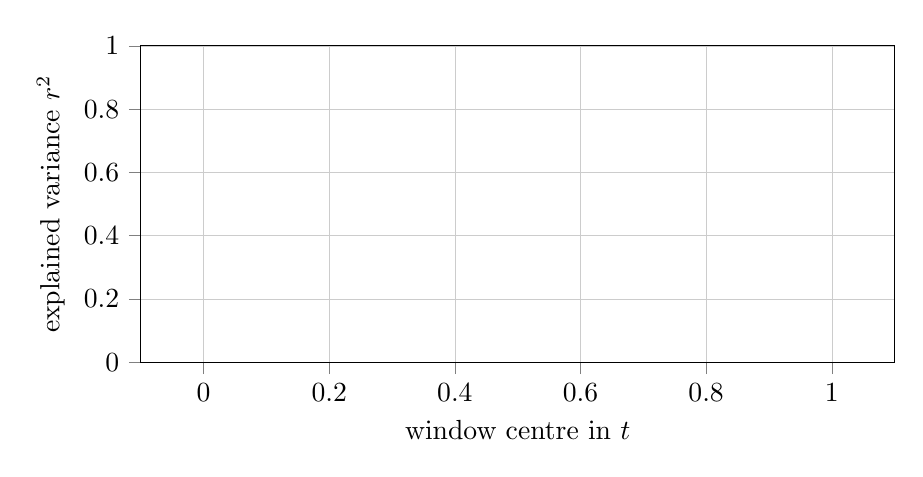
\begin{tikzpicture}
\begin{axis}[floorplot, xlabel={window centre in $t$}, ylabel={explained variance $r^2$},
  legend pos=south west, ymin=0.6, ymax=1.0, height=5.6cm, legend columns=2,
  legend style={font=\scriptsize, draw=gray!40}]
\addplot[mark=*, thick, color=blue!60!black] coordinates {\figscaleMskHi};  \addlegendentry{masked, $P{<}3000$}
\addplot[mark=*, thick, color=blue!35, dashed] coordinates {\figscaleMskLo}; \addlegendentry{masked, $P{<}300$}
\addplot[mark=square*, thick, color=orange!80!black] coordinates {\figscaleRawHi}; \addlegendentry{raw, $P{<}3000$}
\addplot[mark=square*, thick, color=orange!45, dashed] coordinates {\figscaleRawLo}; \addlegendentry{raw, $P{<}300$}
\end{axis}
\end{tikzpicture}
\caption{Masked, the reconstruction is scale-stable at adequate cutoff: $0.9609\to
0.9578$ across a fourfold range in $t$, a decline of $0.003$. Raw, it declines
$0.7551\to0.6728$ at $P{<}300$. So the row-to-row constancy reported in
\cite{threelayer} is held by growing the model with the data and is not evidence of
stability at fixed complexity --- while the stability it asserted is real, and is a
property of the reconstruction away from the staircase.}
\label{fig:scale}
\end{figure}

\section{The battery on the zeros, and an amplification check}\label{sec:zresults}

Criterion~I on the zeros, $K=40$, surrogate by permuting unfolded spacings:

\begin{center}\small
\begin{tabular}{lrrl}
\toprule
Witness & $\sigma_W$ & $z$ & Tier \\
\midrule
arithmetic, $\sum_{p\le29}\langle\cos(\gamma\log p)\rangle^2$ & $3.51\times10^{-4}$ & $\mathbf{499.8}$ & \tier{FUNCTION} \\
lag-1 spacing correlation & $2.16\times10^{-2}$ & $\mathbf{17.6}$ & \tier{FUNCTION} \\
spacing mean deviation & $6.97\times10^{-16}$ & withheld & \tier{FORM\_EXACT} \\
spacing variance & $1.67\times10^{-16}$ & withheld & \tier{FORM\_EXACT} \\
Wigner-shape $L^2$ & exactly $0$ & withheld & \tier{FORM\_EXACT} \\
\bottomrule
\end{tabular}
\end{center}

The split of \cite{ff06e} reproduces --- the arithmetic witness carries the
object-specific influence and the distributional witnesses carry none --- and
Prop.~\ref{prop:degenerate} changes the last three verdicts from \emph{form at
$0.4$--$1.0\sigma$} to \emph{factoring, significance withheld}.

\begin{figure}[ht]\centering
\begin{tikzpicture}
\begin{loglogaxis}[floorplot, xlabel={$N$ (zeros)}, ylabel={$z_{\mathrm{arith}}$},
  legend pos=south east, height=5.2cm]
\addplot[domain=1500:120000, samples=2, dashed, thick, color=gray!60, forget plot]
  {3030*(x/20000)^0.829};
\addplot[only marks, mark=square*, mark size=2.4pt, color=orange!80!black] coordinates {\figamplPub};
\addlegendentry{published \cite{ff06e}}
\addplot[only marks, mark=*, mark size=2.6pt, color=blue!60!black] coordinates {\figamplMine};
\addlegendentry{this record}
\node[anchor=north west, font=\footnotesize, color=gray!40!black] at (axis cs:2400,2700)
  {$z\propto N^{\amplExp}$, fitted on two points};
\end{loglogaxis}
\end{tikzpicture}
\caption{The function signal sharpens with $N$ rather than averaging down, which is the
argument that it resolves structure rather than an artifact. The two published points
fix $z\propto N^{\amplExp}$; extrapolated a decade below the fitted range this predicts
$\amplPred$ at $N=\nZeros$, against $499.8$ measured --- $11\%$ high. The paired caveat
in \cite{ff06e} also holds in the stated direction: the \emph{raw} value is larger at
smaller $N$ ($0.1762$ here against $0.0922$ and $0.0636$), so significance and magnitude
move oppositely. A two-point fit carries no uncertainty estimate, so $11\%$ a decade out
is agreement and not a discrepancy.}
\label{fig:ampl}
\end{figure}

\begin{remark}[A correction to our own earlier figure]
An earlier draft reported this agreement as $4\%$. That used the exponent rounded to
$0.8$, which moves the prediction from $\amplPred$ to $481$ and the discrepancy from
$11\%$ to $4\%$. The exact two-point exponent is $\amplExp$ and the honest figure is
$11\%$. The rounding flattered the comparison and is corrected here.
\end{remark}

\section{A removable artifact}\label{sec:artifact}

Reference~\cite{ff06e} attributes a $0.4$--$1.0\sigma$ residual in its factoring
witnesses to its surrogate path: permute unfolded spacings, re-accumulate, then
interpolate back onto the reference grid. The attribution is correct as to mechanism and
localises further. Two routes from unfolded positions back to heights:

\begin{center}\small
\begin{tabular}{lrrr}
\toprule
Route & spacing mean dev. & spacing variance & Wigner $L^2$ \\
\midrule
Analytic: bisect the monotone $\langle N\rangle$ & $6.2\times10^{-16}$ & $4.4\times10^{-15}$ & exactly $0$ \\
Piecewise-linear between samples & $1.9\times10^{-16}$ & $\mathbf{1.03\times10^{-5}}$ & $\mathbf{3.51\times10^{-4}}$ \\
\bottomrule
\end{tabular}
\end{center}

The artifact requires interpolation between knots, not the round trip. Inverting the
smooth counting function by bisection restores exact invariance, so the residual need
not be explained --- it can be removed. We do not compare the resulting $z$ against the
published $0.4$--$1.0$: ours are $0.16$ and $0.01$, and $z$ here is a ratio of one small
quantity to another, dominated by grid, $N$ and interpolation detail. The finding is
$\sigma_W$ moving from machine epsilon to $10^{-5}$.

\section{Discussion}

The three criteria share a structure. Each identifies a \emph{quotient} the measurement
cannot see past --- the marginal in \S\ref{sec:descent}, the quadratic order of response
in \S\ref{sec:invis}, the location of a residual in \S\ref{sec:gibbs} --- and then asks
whether the quantity of interest is determined by that quotient or lives in its fibre.
Conflating ``not determined by the quotient'' with ``detected'' is the single error
behind all of the omissions reported here.

The amendments cost something. Prop.~\ref{prop:ceiling} converts former \emph{form}
verdicts into \emph{unresolved}, a loss of apparent information. The trade is favourable
for an asymmetric reason: an unresolved verdict can be improved by a better witness or a
larger object, whereas a false \emph{form} verdict cannot be improved, because it does
not know it is wrong. Prop.~\ref{prop:degenerate} replaces a number with a refusal,
which is the harder amendment to accept, since a table with an omission looks weaker
than a table of figures. It is the other way around.

Two of the measurements here are warnings about scalars rather than about instruments.
The order parameter of Fig.~\ref{fig:coex} is exactly computed, carries no numerical
flag, and denotes a state no member of its own distribution occupies; the apparent
scale-degradation of Fig.~\ref{fig:scale} is a correctly computed decline that measures
the grid's proximity to discontinuities rather than the model's reach. Neither failure
announces itself. A number that overflows does not mislead --- it fails loudly.

\section{Scope and claim boundaries}\label{sec:scope}

\textbf{What a \tier{FUNCTION} verdict establishes.} That the witness responds to
structure beyond the chosen quotient, for that object and that construction. Not that it
is correct, meaningful, or evidence for any proposition about the object.

\textbf{No claim about $\zeta$ or the Riemann hypothesis.} Nothing here concerns the
location of zeros off the critical line, the construction of a self-adjoint operator, or
the completeness of the explicit formula as a theorem. Section~\ref{sec:gibbs}
establishes where a \emph{residual} lives, not that a series converges.

\textbf{No claim about continuum $SU(2)$ or about confinement.}
Sections~\ref{sec:lattice}--\ref{sec:firstorder} concern a finite periodic lattice with
a chosen three-character action at zero temperature. The transition is a property of
that action on that lattice; no continuum limit is taken and no finite-size scaling is
performed.

\textbf{Single-implementation results.} Section~\ref{sec:artifact} rests on one
implementation of each route. The qualitative finding is robust to implementation; the
figures are not.

\textbf{Unconverged where stated.} The jump magnitude at $\rho=3.1$
(\S\ref{sec:firstorder}) failed its pre-registered convergence check and is asserted as
a floor only.

\textbf{Where the methods stop.} Criterion~I requires a construction preserving the
marginal while destroying correlation; where none exists the question is well posed and
not answerable by this operator. Criterion~III requires the instrument's failure mode to
be \emph{localised} in a known place; a residual spread uniformly is not separable this
way.

\section{Reproduction}\label{sec:repro}

Seed $20260423$ throughout. Implementation: the \texttt{AISO-UI-for-Ai} tree
(\path{frontend/src/shuffle-knife.ts}, \path{frontend/src/riemann-siegel.ts}, \path{frontend/src/rotor-field.ts}, \path{frontend/src/rotor-dynamics.ts}).
The tree is public at \url{https://github.com/tensorrent/AISO-UI-for-Ai}; the numbers and figures in this document were produced on branch \path{claude/excel-memory-offloading-9ezwrv}, and the four instrument files, the scripts and the lattice test are byte-identical from the generating commits (\texttt{086a0e3}, \texttt{64d9658}) through commit \texttt{3a8e610}, which is the pin. Clone the repository and check it out at that commit,
\begin{center}\small\texttt{git checkout 3a8e610a80575da13ee68649c7a92ba3690be140}\end{center}
then \texttt{npm install} in \path{frontend/} and run the commands below from that directory.

\begin{center}\small
\begin{tabular}{ll}
\toprule
Command & Produces \\
\midrule
\texttt{npx vitest run tests/shuffle-knife.test.ts} & the calibration protocol, \S\ref{sec:calib} \\
\texttt{npx vitest run tests/riemann-siegel.test.ts} & the instrument anchors, \S\ref{sec:gibbs} \\
\texttt{npx vitest run tests/rotor-dynamics.test.ts} & \S\ref{sec:invis}--\ref{sec:battery}, incl.\ the gradient check \\
\texttt{npx tsx scripts/riemann-witnesses.mts} & \S\ref{sec:zresults}, both surrogate routes \\
\texttt{npx tsx scripts/riemann-positions.mts} & \S\ref{sec:gibbs}, \S\ref{sec:scaletest} \\
\texttt{npx tsx scripts/paper-figures.mts} & every figure in this paper \\
\bottomrule
\end{tabular}
\end{center}

The last command emits \texttt{instrument\_floors\_data.tex}, which this document
\texttt{\textbackslash input}s; no figure here is transcribed by hand. Scripts depending
on an anchored instrument exit non-zero if an anchor fails.

\appendix
\section{Dead ends and self-corrections}

Recorded because two of the results above exist only as the residue of an error.

\begin{enumerate}[leftmargin=2em,itemsep=4pt]
\item \textbf{The ascent count was predicted to read \tier{FUNCTION}.} Asserted in
calibration; the assertion failed and the verdict was correct. Became
Prop.~\ref{prop:necessary}.

\item \textbf{An analytic round trip was expected to reproduce the published band.} It
does not --- $\sigma_W$ stays at machine epsilon --- which showed
``re-interpolation'' too coarse a diagnosis and produced \S\ref{sec:artifact}.

\item \textbf{The first destabilising term was link-based and had no threshold at all.}
A term $-\alpha\sum(1-\operatorname{Re}U)$ is not gauge invariant, so it pushes on gauge
directions, which have \emph{zero} restoring force from $\beta$ --- that blindness being
what gauge invariance is. Measured: order parameter at $-1$ by $\rho=0.2$, collapse at
$\alpha=0.4$, no critical ratio anywhere. There is none when the attacked direction has
no stiffness. The face-based term of \eqref{eq:action} is the repair.

\item \textbf{A rounded exponent flattered a comparison} from $11\%$ to $4\%$
(Fig.~\ref{fig:ampl}).

\item \textbf{Two implementations of an unrelated cyclicity figure disagreed by
$3.4\sigma$}, a spread as large as a discrepancy then being claimed against a published
number. The claim was withdrawn until anchors settled it.

\item \textbf{A gauge-invariance control caught a malformed test.} A gauge
transformation was supplied as a generator rather than a function of the vertex;
\texttt{gaugeTransform} queries a vertex more than once, so each call returned a
different rotor and the operation was not a gauge transformation. The control ---
$\langle\operatorname{Re}P\rangle$ must not move --- detected it at $0.9961\to0.4202$.
\end{enumerate}

\begin{thebibliography}{9}
\bibitem{theiler} J.~Theiler, S.~Eubank, A.~Longtin, B.~Galdrikian, J.~D.~Farmer,
  \emph{Testing for nonlinearity in time series: the method of surrogate data},
  Physica D \textbf{58} (1--4), 77--94, 1992. \texttt{doi:10.1016/0167-2789(92)90102-S}.
\bibitem{ff06e} B.~Wallace, \emph{Spectral Rigidity and Shuffled Spacing Discriminant:
  Categorising Spectral Witnesses by What They Respond To} (FF06e), TensorRent, 2026;
  amendment of 24 September 2026.
\bibitem{threelayer} B.~Wallace, \emph{Density, Positions, Spacings: A Three-Layer
  Decomposition of the Riemann Zeros}, TensorRent, 2026; amendment of 24 September 2026.
\bibitem{edwards} H.~M.~Edwards, \emph{Riemann's Zeta Function}, Academic Press, 1974
  (Riemann--Siegel formula, Ch.~7).
\bibitem{wilson} K.~G.~Wilson, \emph{Confinement of quarks},
  Phys.\ Rev.\ D \textbf{10}, 2445--2459, 1974.
\end{thebibliography}

\vspace{1em}\noindent\rule{\linewidth}{0.4pt}\\[2pt]
\small\textbf{Contributions.} The marginal-matched discriminant, the form/function
vocabulary and the finding that a battery of agreeing witnesses may be one reading
refracted are due to \cite{ff06e}; the three-layer decomposition and its completeness
reading to \cite{threelayer}. Criterion~I's three propositions and quotient recasting,
the four-tier procedure, the three-character action and its validation, criteria II and
III, both instruments, all six figures and the artifact localisation are this record's.
Byline deliberately unset. Every figure is emitted by the measurement that produced it;
no number here is quoted from memory or from a source not opened.

\end{document}
